\section{Discussion}
\label{ch61:discuss}

In this section I summarise and discuss the findings from the previous chapters, relating them to emerging related work and future directions.

\subsection{Making a predictable ecosystem of FAIR digital objects}
\label{ch61:ecosystem}

The main advantage of scholarly researchers publishing \emph{FAIR data} is to enable machine actionability \cite{Wilkinson 2016}, which again will accelerate further research, such as through computational workflows. 
In practice, data publishing is largely approached either by depositions in general and institutional repositories for Open Data such as Figshare and Zenodo \cite{Dillen 2019}, or to specialized domain-specific repositories such as in biodiversity \cite{ch8-7}. 

European research infrastructures supporting Open Science practices are coalescing their services to form the European Open Science Cloud (EOSC) \cite{10.2777/940154}, which are embracing FAIR principles \cite{Mons 2017} and building a common framework for interoperability \cite{eosc-interop-framework}. 

While existing practices for implementing FAIR have relied on the Linked Data stack, that is just one possible technology to achieve the benefits of interoperable machine actionability \cite{Mons 2017}. 

Chapter \ref{chapter:fdo} explored the emerging concept of \emph{FAIR Digital Objects} (FDO) \cite{Schultes 2019} as a potential distributed object system for FAIR data, comparing its proposed principles and current practices with the established Linked Data approach. 
As detailed in section \vref{ch3:fdo}, FDO defines a handful of constraints and guides for a predictable way to organise complex machine actionable digital entities. 

Conceptually FDO can clearly be useful for realizing FAIR principles with more active digital objects that can form a consistent ecosystem, but this opens many questions on actual FDO implementations with regards to protocols and standards.

\subsubsection{Linked Data need more constraints and consistency to be FAIR}
\label{ch61:constraints}

Examined in section \vref{ch3:ld}, the principles of \emph{Linked Data} emerged from the Semantic Web as a data-centric view with a focus on navigation and cross-site interoperability, rather than say elaborate logical inferencing systems using ontologies.  
Yet the bewildering landscape of technology choices for using RDF in data platforms means that the developers suffer and still face a steep learning curve. 
For clients consuming Linked Data from multiple sources -- \emph{Linked Data Mashup} \cite{Tran 2014} -- the situation is still baffling in that relatively small differences in identifiers, vocabularies and usage patterns across deployment result in incompatibilities that may require platform-specific workarounds and mappings \cite{Millard 2010}. 

The ecosystem of FAIR tooling is not currently mature enough to support Linked Data consumption in a user-friendly and efficient way \cite{Thompson 2020}, although recent metrics and tools for assessing \emph{FAIRness} \cite{Wilkinson 2018} can assist both data providers and consumers. 
Evaluations by EOSC has since found that FAIRness metrics can vary widely across the different assessment tools for the same data resource \cite{10.5281/zenodo.7463421}, showing that further definitions of conventions and practices are needed for consistent Linked Data publishing and consumption. 

Making the FAIR principles achieve practical benefits for researchers and platform developers thus requires more specific constraints and broader consistency.

\subsubsection{FDOs as a distributed object system on the Web}
\label{ch61:distributed}

The framework-based comparisons in section \vref{ch3:results} considered the implementation details of both FDO and Linked Data, and evaluated to what extent either can be considered a global distributed object system. 
The findings from this research show that FDO recommendations can benefit FAIR thinking to build machine actionable ecosystems and provide stronger promises of consistency and predictability across data platforms. 

These comparisons highlighted that the Web on the other hand has a flexible, scalable and mature technology stack, which can form a solid basis for implementing FDO. 
However, if such implementation is to use Linked Data technologies, these must be constrained sufficiently in order to practically realize such an ecosystem within the FDO guidelines and without degrading the developer experience.


\subsubsection{FDOs can be implemented on the Web using Signposting}
\label{ch61:signposting}

Section \vref{ch2:meeting-fdo-principles-using-linked-data-standards} explored how the FDO principles can be achieved for Linked Data as further constraints on existing standards.
As chapter \ref{chapter:fdo} has highlighted throughout, there are many technical details remaining to be specified for FDO it to be consistently implemented according to its own principles.

If such conventions need to be evolved and specified no matter the protocol basis for FDO, this chapter argued, then it would be intuitive to build FDO on the mature Web stack, unless there was an compelling argument for alternative protocol stacks having other advantages.\footnote{
  For instance, a de-centralized, resiliant architecture and long term preservation was the motivation for the design of the Interplanetary File System (IPFS) as a \emph{Decentralized Web} \cite{Trautwein 2022}.
}

Section \ref{ch2:discussion} found that the basis of Web-based FDOs can be built using only Signposting \cite{vandesompel2015,Van de Sompel 2022}, adding a couple of non-intrusive HTTP headers that are agnostic to metadata standards and serializations. An implementation of such Web-based FDOs was shown in section \ref{ch4:lightweight-fdo}. 

The Signposting approach has also been highlighted both by EOSC \cite{10.5281/zenodo.7463421} and as a possible FDO configuration type \cite{fdo-ConfigurationTypes}.
The FAIR-IMPACT project launched an \footurl{https://fair-impact.eu/1st-open-call-support-closed}{open call} where 14 participating institutions participated to help build support for Signposting \cite{soilandreyes2023b} in data repositories and platforms.



\subsection{RO-Crate as a developer-friendly approach}
\label{ch61:crate}

As pointed out in section \vref{ch3:ld-web}, while Linked Data is a powerful and flexible approach to publishing structured data on the Web, the developer experience of using Semantic Web technology still needs simplifications, like reducing number of choices for vocabularies and serialization formats. 

Chapter \vref{chapter:ro-crate} introduced \emph{RO-Crate} as a practical implementation of the FAIR principles for the purpose of packaging data alongside structured metadata.
The approach builds on best practices for Linked Data, however RO-Crate specifications are example-driven with simple interrelated JSON structures, and primarily use a single, general purpose vocabulary. 

This way of ``Linked Data by stealth'' means that developers don't need to be concerned about RDF implementation details, although they can at their option take advantage of RDF knowledge graph technologies like SPARQL (section \vref{ch5:linkeddata}).
Extension points are well defined, and although extending RO-Crate do require some RDF knowledge like defining namespaces, reasonable examples and vocabulary repositories are provided by RO-Crate --  developers do not for instance need to learn about ontologies nor need to deploy a web service serving multiple RDF serialisations for every described entity.



\subsubsection{Just enough Linked Data}
\label{ch61:justenough}

An important lesson from this work then is to use ``just enough'' Linked Data for the desired level of interoperability and knowledge representation.
While previous efforts to `FAIRify' largely have been concerned about representing the data values using an RDF data model, this can lead to significant effort needed in developing ontologies and vocabularies. 

RO-Crate is using schema.org \cite{schema.org} as its base vocabulary, and tries to follow its philosophy of building a lightweight semantic structure by associating many free text attributes to the same node, rather than making elaborate interconnected semantic objects.
For instance, while a \texttt{Person}'s \texttt{affiliation} ideally goes to a \texttt{Organization} with it's own URL and other attributes, in some cases, a free text string is all information available, and this can be used cirectly as the \texttt{affiliation}. 

With retrospect we can say that this reduction in semantic rigidity compared to use in OWL ontologies is a move back to the simplicity of early RDF as an open-ended model (see section \vref{ch3:semweb}), where a property can be used to point to almost anything, and RDF authors are free to use almost any term.

Another aspect that is not highlighted well in ontologies is where to stop in the formal knowledge representation of an object.
In schema.org, many properties like \url{http://schema.org/license} are defined as having the \emph{range}\footnote{Expected type of object \cite{w3-rdf-schema}, however note that schema.org uses \url{http://schema.org/rangeIncludes} instead of \texttt{rdfs:range}, to permit multiple alternatives without the need for a union class.} of either \footurl{http://schema.org/CreativeWork}{\texttt{CreativeWork}} or \footurl{http://schema.org/URL}{\texttt{URL}}, hinting that the licence is not required to be explained as another entity with further properties, but that the attribute's primary purpose is navigation or identification. 

This would be a key aspect of Linked Data, which traditionally have had the rather undefined convention of ``follow your nose'' navigation -- a client may attempt to request any node identifier (if it's a URL), and if, with content-negotiation, it returns some RDF, then that could be integrated into a joint knowlege graph, hopefully adding more description of that node, although possibly using other vocabularies.
However, ontologies used in Linked Data have not commonly indicated navigation waypoints as done in Schema.org, simply defining a property's range as a given class leaves it undefined if documents were expected to explain that node or link to its explanation. One notable exception is the Data Catalog Vocabulary (DCAT)\footnote{Although the \url{http://schema.org/Dataset} type used by RO-Crate's root entity is derived from DCAT, RO-Crate does not assume a corresponding data catalogue on the Web.} \cite{DCAT2 2020} which have navigational properties like \texttt{dcat:landingPage} (to a \texttt{foaf:Document}) and \texttt{dcat:downloadURL} (to any \texttt{rdfs:Resource}).

% Should we discuss why not DCAT?

\subsubsection{Embedding contextual information reduces need for navigation}
\label{ch61:contextual}

A divergence from common Linked Data practices is that our RO-Crate approach is making a self-described container.
Rather than assume that information will always be available from the referenced URIs, and requiring clients to crawl their way through the many identifiers to see which ones contain more information, the RO-Crate contains a minimal description of each referenced contextual entity (section \vref{ch5:contextualentities}). 

This has multiple purposes:

\begin{itemize}
    \item Simplify user interfaces, e.g. show a human-readable label and type before the user chooses to click the link.
    \item Vocabulary adaptation, for instance describing with schema.org in the crate, what was expressed in FOAF vocabulary at the URI.
    \item Unify descriptions of semantic artefacts and web pages. 
          Making ``ad-hoc'' semantic artefacts within the crate where none exited beforehand.
    \item Embed ``as of at time of writing'' descriptions for longevity. 
          An RO-Crate is self-contained and can be archived independently, and embedding contextual information reduces cross-organizational service dependencies (at the risk of outdated information).
\end{itemize}

Several of these reasons are also organizational in nature, reflecting back on the EOSC Interoperability Framework (section \vref{ch3:eosc-interoperability-framework}) -- rather than requiring for instance the Research Organization Registry \footurl{https://ror.org/}{(ROR)} to add Linked Data representations of organizations, one can be made ad-hoc by the RO-Crate's author, and contained by the crate as a contextual entity. 

This ability to describe a referenced entity locally is also a workaround for the chicken-and-egg problem of creating and linking Linked Data resources that vocabulary-wise are cross-related both ways. For instance orcid.org recently added schema.org content negotiation, but \emph{after} RO-Crate started describing people using the \url{http://schema.org/Person} type and ORCID identifiers.\footnote{
  One of my earlier code contributions to ORCID already established content-negotiation to RDF -- but using the classical FOAF vocabulary \cite{FOAFVocabularySpecification}.
  Slightly inconsistent with Semantic Web principles, the registry is currently returning \emph{Person} descriptions in different semantic models depending on the requested serialization. \\
  \url{https://github.com/ORCID/ORCID-Source/blob/main/CONTENT_NEGOTIATION.md}} 


\subsubsection{FDO ecosystems need to permit flexible references}
\label{ch61:references}

When reflecting on the above contextualization from the propositions of FAIR Digital Objects as covered back in chapter \ref{chapter:fdo}, we can predict a problem if every reference from an FDO must go to another pre-existing FDO (or at least a registered PID), in that there must then be a linear order of FDO creation within an ecosystem of compatible FDO types.
A strict reading of the FDO principles means implementations cannot utilise the established human-readable Web for bootstrapping.
This risks large cross-organizational delays with a stronger need for collaboration and coordination, or alternatively, starting with a smaller FDO data models that can gradually evolve to add more navigation, when and if registries appear with FDO interfaces. 

The emphasis on strong typing in FDOs also means that seemingly incompatible types (for instance developed by the biodiversity community vs. those from genomics communities) lead to a split of the PID space of referencable objects from a given type of FDOs.  Counter to this, the current FDO recommendations for attributes and types \cite{fdo-ImplAttributesTypesProfiles} do not require specification of the \emph{range} of an attribute to be a PID of an FDO, and as current FDO type declarations have been relatively lightweight (textual descriptions only), they are flexible enough to permit URLs to any Web resource or existing Linked Data concepts.  

There is a concern however that some FDO serializations using the Handle system and key-value attributes cannot distinguish between string literals and object references.
Combined with the use of PID references expressed as handles rather than as a URIs (e.g. \texttt{21.14100/2fcf49d3-0608-3373-a47f-0e721b7eaa87} instead of \url{https://hdl.handle.net/21.14100/2fcf49d3-0608-3373-a47f-0e721b7eaa87}), this means that machine actionability suffers, in that the string value is not typed to what kind of reference it may or may not be, or in what PID system. Compare this with listing \vref{ch3:triples} where the RDF syntax distinguishes literal strings from object references -- in Handle-based FDOs, machine-actionable navigation is only possible by understanding the attributes of the FDO type, yet as highlighted in the previous paragraph these type definitions are not directly machine-actionable themselves.

In schema.org we find a similar challenge with properties permitting both string values and object references. \url{http://schema.org/keywords} is perhaps the most ambiguous, as it permits \texttt{Text}\footnote{To conflate matters, the \texttt{keywords} property can be repeated, but also allows multiple keywords within a single comma-separated string.}, but also \texttt{URL} or \texttt{DefinedTerm}.
The two latter cases are both intended for referencing controlled vocabularies, with the distinction that a \texttt{DefinedTerm} is defined explicitly within the referenced object, while the defined term is implied if only the URL is provided.
JSON-LD contexts have the possibility of enforcing object references (\texttt{"@type: "@id"}), but this cannot be used in this case as freetext strings are also permitted.
The result is that a freetext keyword that just looks like a URL cannot be distinguished from an intended URL reference, similar to the FDO Handle example in the previous paragraph.

In order to reduce such ambiguity and multiple developer choices, in RO-Crate all object references are in JSON-LD object form, and the RO-Crate context do not have any \texttt{@type} shortcuts for implicit references.
RO-Crate 1.2 will also recommend that \footurl{https://www.researchobject.org/ro-crate/1.2-DRAFT/metadata.html\#common-principles-for-ro-crate-entities}{all entities} have a type, identifier and human-readable name. 


\subsubsection{Profiles restrict general flexibility to gain specific predictability}
\label{ch61:profiles}

Section \vref{ch5:inuse} showed how RO-Crate is adopted by different scientific domains. 
Since the publication of the corresponding manuscripts in chapter \ref{chapter:ro-crate}, RO-Crate has also been used by the \footurl{https://www.researchobject.org/ro-crate/in-use/LDaCA.html}{Language Data Commons of Australia} \cite{LREC2022} building language corpa, \footurl{https://www.researchobject.org/ro-crate/in-use/survey-ontology.html}{Survey Ontology} \cite{surveyOntology} describing surveys, \footurl{https://nfdi4plants.org/content/learn-more/annotated-research-context.html}{DataPlant} for plant experiments, \footurl{https://w3id.org/cpm/ro-crate}{distributed provenance} of biological specimens \cite{Wittner 2020,Wittner 2023,Wittner 2023b}, \footurl{https://w3id.org/ro/doi/10.5281/zenodo.6913045}{COVID-19 causal inferences} to compare public health interventions internationally \cite{Meurisse 2023}, and \footurl{https://w3id.org/5s-crate/0.4}{Trusted Research Environments} for controlled workflow computation on sensitive health data. Several of these use cases have also expanded RO-Crate with additional terms from schema.org or defined in corresponding RO-Crate profiles. The span of these domains shows that RO-Crate is flexible for a range of use cases and can be adopted by developers not familiar with Semantic Web technologies.

The discussion of strictness vs flexibility in section \vref{ch5:strictness-vs-flexibility} highlighted the tension between a flexible open-ended model and the predictability needed to consistently create and consume content expressed by the model.
While RO-Crate itself can be seen as a restriction of the more open-ended JSON-LD and schema.org, its extensibility points still allow different use cases to expand on those conventions.  

Section \vref{ch5:profiles} detailed how semi-formalized profiles can be gradually formed to at first \emph{duck-type} a class of RO-Crates that have similar properties.
Later work has formalized this as \footurl{https://www.researchobject.org/ro-crate/1.2-DRAFT/profiles}{Profile Crate} to capture the profile itself as a separate crate. This have now evolved to use the W3C Profiles Vocabulary \cite{dx-prof} to explicitly link to vocabularies, mappings and importantly constraints expressed as RDF Shapes \cite{fdo-collections}. 
This turns RO-Crate profiles into machine-actionable type definitions, from which existing RDF tooling can do for instance validation. 
Figure \ref{ch61:fig:profilecrate} shows how the usage of \emph{roles} within the profile crate indicates the purpose of the constituent parts.
Roles are here particularly important as many of these Semantic Web resources are expressed in the same file format (e.g. \texttt{text/turtle}) and may be used for different purposes (e.g.
SKOS is used to represent either a \emph{mapping} or a \emph{vocabulary} \cite{w3-skos-primer}).

\begin{figure}[htb]
    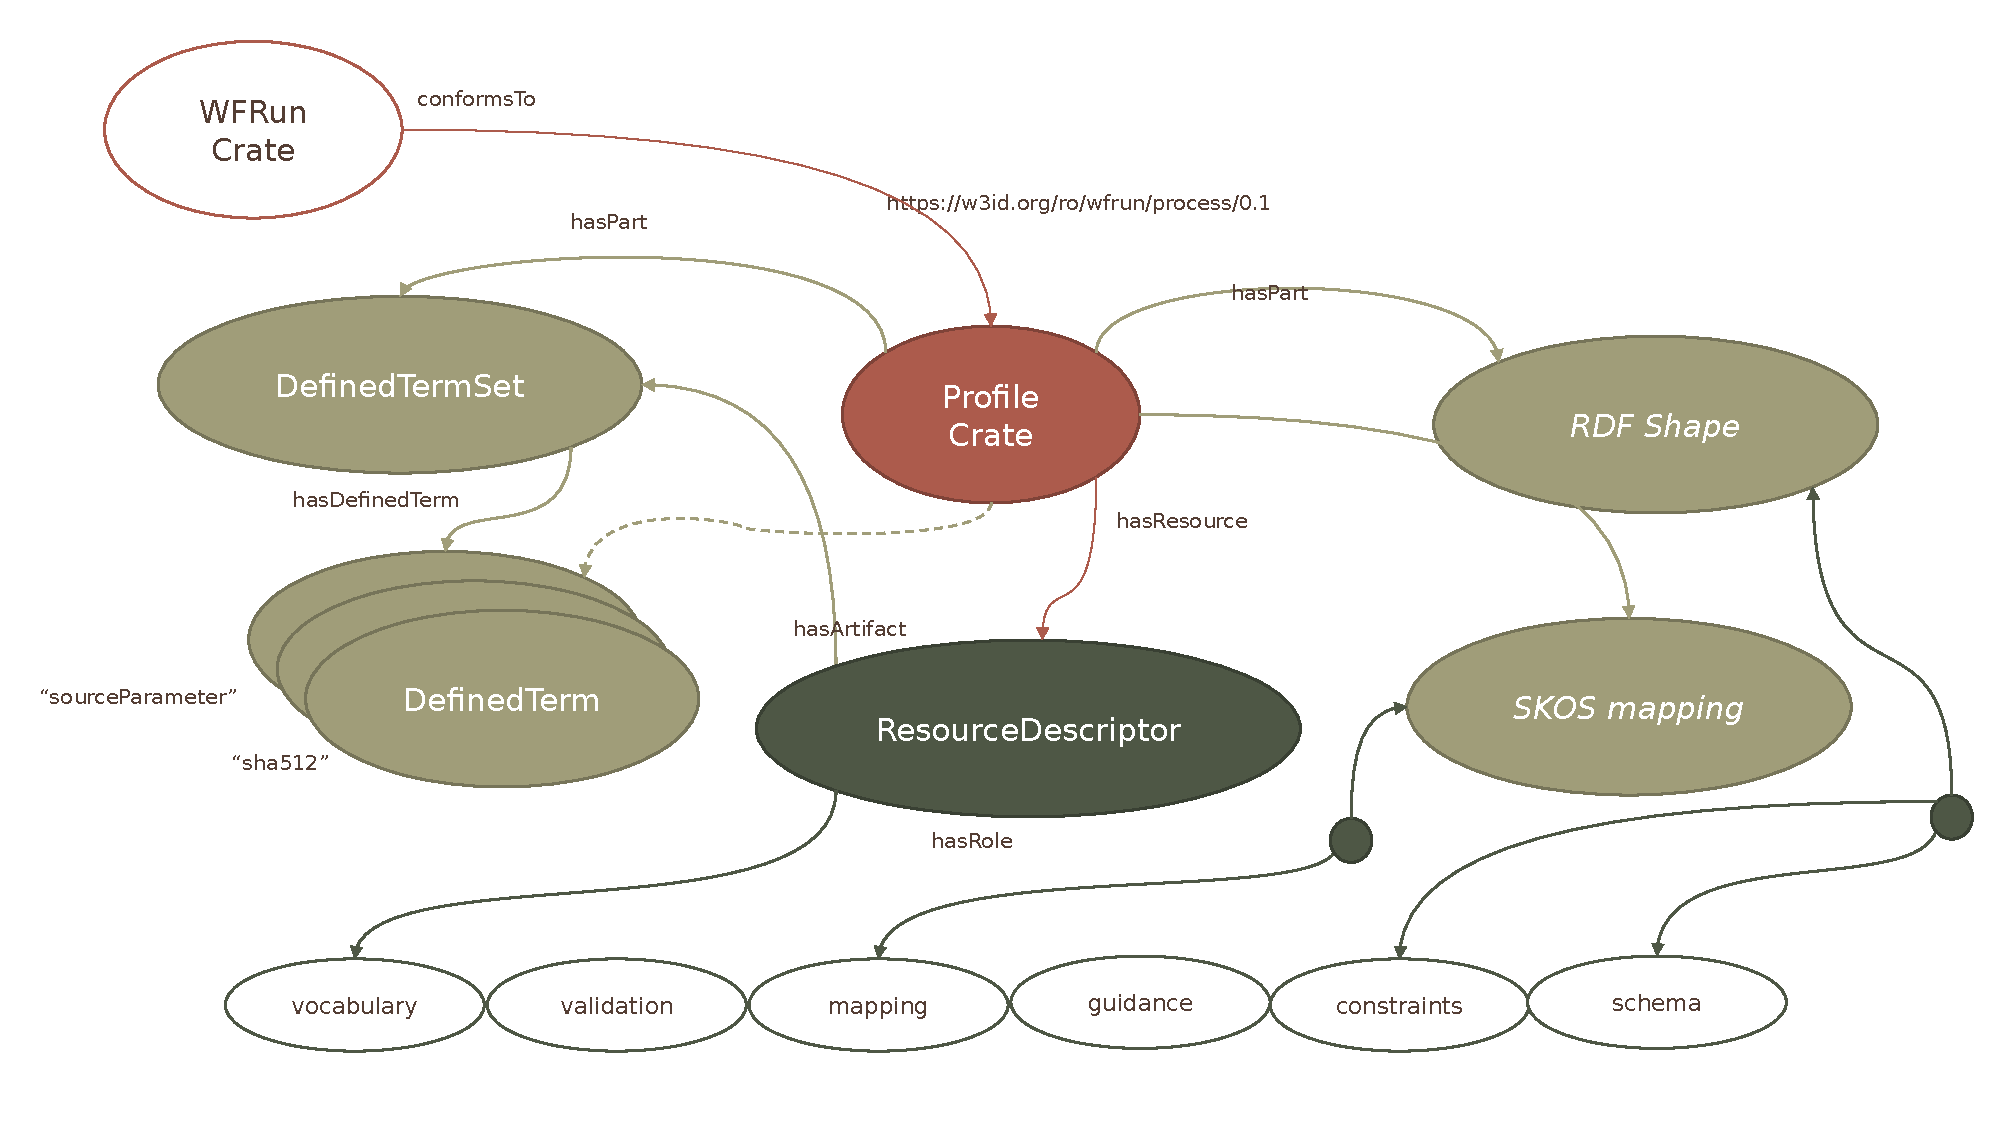
\includegraphics[width=\textwidth]{figures/ch09/profile-crate.pdf}
      \caption[Example of Profile Crate]{\textbf{Example of Profile Crate for Workflow Run Crate}. 
      An RO-Crate \emph{WFRun Crate} declares conformance with a given RO-Crate profile. 
      Resolving the profile URI retrieves the \emph{Profile Crate}, which parts include an \emph{RDF Shape}, an \emph{SKOS mapping} and a \emph{DefinedTermSet}. 
      By using the indirection of \emph{ResourceDescriptor} from the Profiles Vocabulary \cite{dx-prof}, the roles of each of these artefacts are defined, e.g. \emph{constraints}. 
      The embedded \emph{vocabulary} as a \emph{DefinedTermSet} defines ad-hoc terms like \emph{sourceParameter} used by the Workflow Run Crate\footnotemark~ profile \cite{workflow-run-crate}.
      }
    \label{ch61:fig:profilecrate}
  \end{figure}
\footnotetext{\url{https://w3id.org/ro/wfrun/process/0.2}}

While profiles are at first lightweight indicators of common conventions for a class of crates (which may be implicit or explicit), they can be gradually formalized in a \emph{eat own dogfood} way through another RO-Crate, optionally taking advantage of existing Semantic Web technology that can enable for instance strict validation of domain-specific RO-Crates.


\subsubsection{One vocabulary is not enough, but one profile may suffice}
\label{ch61:oneprofile}

RO-Crate relies heavily on \cite{schema.org} as its main vocabulary, but as highlighted in section \vref{ch5:futurework} and \vref{ch61:profiles}, domain-specific usage will eventually need to define their own terms in order to be specific enough for their use cases. However, we have found it is important to ensure a developer-friendly approach when specifying such profiles for RO-Crate -- earlier work on \footurl{https://www.researchobject.org/ro-crate/1.1/appendix/jsonld.html\#adding-new-or-ad-hoc-vocabulary-terms}{ad-hoc terms} in RO-Crate used a simple CSV approach to be added to the \footurl{https://github.com/ResearchObject/ro-terms}{ro-terms} namespace.  

As with other aspects of RO-Crate, there is a gradual approach towards Linked Data practices. While conventional wisdom in Semantic Web would be to sit down and make your own ontology following design patterns \cite{Blomquist 2009,Poveda 2010} and best practices for deployment \cite{Matentzoglu 2022}, in RO-Crate philosophy that would be more of a last resort. The middle of the ground is therefore adding the ad-hoc vocabulary directly to the profile crate, as shown in figure \vref{ch61:fig:profilecrate}. In this approach a single profile URI can, through Linked Data and Signposting, play the role of:

\begin{itemize}
  \item Human-readable documentation of conventions (negotiated to HTML preview)
  \item List of software and repositories the profile is intended for
  \item List of additional schema.org types and properties utillised by the profile
  \item Indication of which content is expected in the crate (e.g. a Workflow)
  \item Validation of a manifest conforming to the profile
  \item Vocabulary definitions of additional terms
  \item JSON-LD context which namespaces the additional terms  (as any JSON-LD document can also be a JSON-LD context \cite{w3-json-ld})
\end{itemize}

It should be reasonable to expect developers able to make RO-Crates with their own additional terms to also be able to make a lightweight Profile Crate once those terms have stabilised. Developers with deeper familiarity with Semantic Web technologies can expand the profile capabilities to use existing ontology methodologies, in which case it would be preferrable to aggregate separate semantic artefacts from the Profile Crate rather than embedding them in the RO-Crate Metadata File.

In the FAIR-IMPACT project we are evaluating if the Profile Crate approach is also suitable for FAIR publishing of semantic artefacts themselves, e.g. ontologies and mappings. This is an attractive proposal because such artefacts are also becoming multifaceted, with multiple formats and profiles (e.g. an ontology expressed with OWL2 RL in RDF Turtle syntax), documentation and similar attribution and provenance challenges that RO-Crate resolves.

\subsection{Future RO-Crate directions}
\label{ch61:rocratefuture}
In this section we consider future directions for RO-Crate and ongoing RO-Crate adaptations not covered by section \ref{ch5:packaging-research-artefacts-with-ro-crate}.


\subsubsection{User applications are needed for researchers to generate FAIR Research Objects}
\label{ch61:applications}

RO-Crate and its best practices can be considered a type of \emph{middleware} used by application developers to capture and transmit metadata and relate data files that together form some tangible unit (a \emph{Research Object} \cite{Bechhofer 2013}). While RO-Crate have already been implemented by several repositories and applications such as workflow systems, it is important to also consider the role of user applications in order to increase adoptation of FAIR research objects by scholars in general.

Futher work by the RO-Crate community has created more user-fronting tools such as \footurl{https://github.com/oeg-upm/ya2ro}{ya2ro}, which given metadata and identifier in a YAML\footnote{
  YAML is a file format with the same data model as JSON, but with a more readable syntax, e.g. using indentation instead of quoted strings.  \url{https://yaml.org/}} 
file can retrieve contextual metadata from ORCID, GitHub and DOI registries and build and publish a completed RO-Crate \cite{ya2ro}.   
While this technology still requires some understanding of editing, it is intended to be more approachable to data scientists and for use with simple Web publishing platforms like \footurl{https://pages.github.com/}{GitHub Pages}. The GitHub Action \footurl{https://github.com/marketplace/actions/ro-crate-preview}{ro-crate-preview} also automate HTML preview generation of crates on GitHub Pages.

The repository \footurl{https://www.rohub.org/}{ROHub} \cite{ch5-48} has recently added RO-Crate import and export \cite{Fouilloux 2023}, and provides both a browseable repository for publishing crates, but also interactive and collaborative editing of its metadata. 
In this use case, RO-Crate plays the role as an exchange and archiving format, as the hub stores the crates in general-purpose repositories Zenodo and B2Share which do not have the facility to keep the granular metadata expressed within the RO-Crate metadata file. As detailed in \cite{Fouilloux 2023}, a series of templates assist users in creating research objects with particular content and annotations. 

The \footurl{https://schema.org/docs/schemas.html}{Crate-O} tool has been developed by Language Data Commons of Australia \footurl{https://ldaca.edu.au/}{(LDaCA)} as a general-purpose RO-Crate editor and successor to Describo \cite{ch5-78} and Describo Online \cite{ch5-77}. 
This tool can describe any folder and resources from the Web as an RO-Crate, supporting any schema.org type and property, pluggable with any rdfs vocabularies \cite{w3-rdf-schema}. 
Notably this tool is also intended for creation of such vocabularies, and is thus a lightweight user interface for building a Profile Crate (section \vref{ch61:profiles}) using Schema.org style Schemas\footnote{
  It is notable that schema.org's own vocabulary definition use rdfs directly for Linked Data interoperability, 
  rather than its own \url{http://schema.org/Class}, \url{http://schema.org/Property}, or the SKOS-like \url{http://schema.org/DefinedTerm}. 
  On property definitions, SoSS use \url{http://schema.org/domainIncludes} and \url{http://schema.org/rangeIncludes} to avoid union classes for alternative domain/range types, which can clutter OWL/RDFS equivalent properties.} 
\footurl{https://schema.org/docs/schemas.html}{(SoSS)}.


\subsubsection{Executable paper using RO-Crate}
\label{ch61:livepublication}

\footurl{https://livepublication.github.io/LP_Pub_LID/}{LivePublication} \cite{Ellerm 2023} is a proof of concept of an \emph{executable paper}, which interactive visualization and statistical calculations can be regenerated on the fly taking into consideration data sources updated after the paper's publication date. A \footurl{https://livepublication.github.io/LP_Pub_OrchestrationCrate/}{corresponding RO-Crate} is the mechanism to enable this execution on the Globus infrastructure through individual RO-Crates and containers for each computable element of the paper.

This novel approach shows how it is possible to use RO-Crate as an machine-actionable object, which do not rely on bundling an underlying workflow representation in an existing workflow language.  

\subsubsection{Web-based FDOs can use RO-Crate for its metadata}
\label{ch61:webfdo}

Section \vref{ch4:lightweight-fdo} argues that many of the FDO requirements \cite{fdo-RequirementSpec} for metadata can be implemented as \emph{RO-Crate FDOs} (section \vref{ch8:fair-packaging-of-researchworkflow-objects-with-ro-crate}), with FAIR Signposting \cite{vandesompel2015,Van de Sompel 2022} assisting navigation from persistent identifiers, and the RO-Crate containing the metadata. 

This approach was first implemented in the repository WorkflowHub \cite{Goble 2021,wittenburgFAIRDigitalObject2022b}, and in the FDO Forum \cite{Van de Sompel 2023} suggests RO-Crate with Signposting as a modern update to his OAI-ORE\footnote{OAI-ORE was also used by earlier Research Object approaches \cite{Belhajjame 2015,ch5-111} to capture the aggregation aspect of ROs.} approach from 2008 \cite{ORESpecificationAbstract}.  
RO-Crate FDOs are being further developed within the Horizon Europe projects \footurl{https://eurosciencegateway.eu/}{EuroScienceGateway} \cite{10.5281/zenodo.7152762} and \footurl{https://fair-impact.eu/}{FAIR-IMPACT} \cite{10.5281/zenodo.7157647}.

RO-Crate FDOs complements the findings of section \vref{ch61:signposting}, in that RO-Crate provides FDO with a generic metadata framework and a serialization that can work both for FDOs on the Web and with legacy Handle/DOIP approaches --  this metadata role for RO-Crate in the FDO ecosystem is also highlighted by \cite{Wittenburg 2023b}.

Some extra considerations is rightly needed on identifiers to reduce relative paths challenges with  RO-Crate FDOs -- for this purpose, the next specification \cite{rocrate1.2} introduce a distinction between an \footurl{https://www.researchobject.org/ro-crate/1.2-DRAFT/structure.html\#attached-ro-crate}{attached RO-Crate} (\emph{has some root directory containing other files referenced by relative paths, possibly archived in a ZIP or exposed on the Web}) and a \footurl{https://www.researchobject.org/ro-crate/1.2-DRAFT/structure.html\#detached-ro-crate}{detached RO-Crate} (\emph{no defined root directory, all references are absolute}). 
This \emph{detached} style is suitable for an FDO architecture, even for use within APIs which do not lend themselves to relative path references (such as DOIP-over-HTTP \cite{DOIPAPIHTTPa}).
RO-Crate 1.2 also define methods for \footurl{https://www.researchobject.org/ro-crate/1.2-DRAFT/appendix/relative-uris.html}{converting between attached/detached} crates using standard JSON-LD tooling, showing another advantage of using Linked Data as basis for RO-Crate. 


\paragraph{How FAIR are RO-Crates?}
\label{ch61:fair-crates}

FAIROs \cite{FAIROs} is a framework for calculating a ``FAIRness'' score for research objects. For RO-Crate evaluation this puts additional requirements on the use of persistent identifier for the RO-Crate, and that the core metadata of the crate (e.g. licensing) is provided. These aspects are important for ensuring FDO machine actionability of RO-Crates.


\subsubsection{RO-Crate can capture collections of digital objects}
\label{ch61:collections}

RO-Crate has also been proposed as a generic mechanism for FDO Collections \cite{fdo-collections}, as an aggregator of FDOs by their PIDs. Such collections add a similar challenge in FDO as in Linked Data, in that clients may need to resolve an excessive number of persistent identifiers (see section \vref{ch20:avoid-lots-of-requests}) to FDOs which may be of different semantic types. 
Using a detached RO-Crate for such collections, the bibliographic metadata of each PID can be directly embedded and normalized to a single vocabulary, reducing client needs for recursive queries and type mappings. 
 
Work on building large data citations as a ``reliquary'' -- a \emph{container of persistent identifiers (PIDs)} \cite{Buck 2022} -- started from the earth science domain with AGU's \footurl{https://data.agu.org/DataCitationCoP/}{Data Citation Community of Practice} and continues in RDA's \footurl{https://www.rd-alliance.org/groups/complex-citations-working-group}{Complex Citation Working Group}. In this approach RO-Crate is being considered as a promising implementation to capture large number of citations along with minimal metadata, including licensing and attribution. Here a main motivation is to avoid excessive lists of data citations for scholarly publications following processing of aggregated datasets from repositories such as GBIF \cite{ch8-7}, while still propagating each dataset's FAIR metadata (as required by the Creative Commons Attribution licence) through the indirection of a collection. There is a potential overlap with workflow run provenance, although a workflow is not required by reliquaries.


\subsubsection{RO-Crate in data lakes}
\label{ch61:datalakes}

Knowledge Enhanced Digital Objects \footurl{https://github.com/luoyu357/KEDODataLake}{(KEOD)} \cite{Luo 2022} is an experimental approach of building a data lake using a combination of knowledge graphs, RO-Crate and PID records \cite{Luo 2023}. This is effectively an FDO implementation: A KEDO PID is a Handle that identifies a KEDO Object, described using a KEDO RO-Crate. This crate again has \emph{internal RO-Crate}s as parts, which records a combination of \emph{Features} and \emph{Insights}. The distinction is that features are mainly fixed at digital object creation and considered directly describing the object's nature, while insights can be discovered later from further processing and linkage. This approach solves a mutability problem in FDOs, as the KEOD system only allows insights to be added along with provenance that connect PIDs when KEDOs evolve. Files in a KEDO RO-Crate are stored locally, and each recorded with a Handle PID within the crate.

This KEOD setup of multiple graphs forming a single knowledge unit can be considered analoguous to nanopublications \cite{Kuhn 2021} but for FDOs. Indeed using nanopublication to capture FDOs of digital twins has also been proposed \cite{10.3389/data.2022.883341}, that however use a different distributed architecture where the PIDs for nanopublications are generated by cryptographically hashing their content \cite{Kuhn 2021}.


\subsubsection{Distributed FAIR Digital Objects using Blockchain}
\label{ch61:dpid}

The \footurl{https://docs.desci.com/}{DeSci Nodes} system has been developed by the \footurl{https://www.descifoundation.org/}{DeSci foundation}, where \footurl{https://www.dpid.org/}{dPID} (distibuted Persistent Identifier) act  as an overlay of the Interplanetary File System (IPFS) \cite{Trautwein 2022}. Users can interact with the DeSci platform for building and publishing Research Objects, and the \footurl{https://docs.desci.com/learn/open-state-repository/metadata}{DeSci metadata} are exposed as a \footurl{https://www.researchobject.org/ro-crate/1.2-DRAFT/structure.html\#detached-ro-crate}{detached RO-Crate} with IPFS references (see \footurl{https://beta.dpid.org/46?jsonld}{example dPID 46}).

This is a novel FAIR Digital Object implementation that challenges both the traditional centralised FDO approach using the Handle system, as well as the mostly Web-based RO-Crate ecosystem covered in section \vref{ch5:packaging-research-artefacts-with-ro-crate}. The use of detached crates has also been \footurl{https://www.researchobject.org/ro-crate/in-use/LDaCA.html}{Language Data Commons of Australia Program}, where RO-Crate is part of navigating API resources, rather than a standalone publication on the Web. In both of these approaches, additional FDO measures such as using persistent identifiers and validation against profiles become important. 




\subsection{Workflow}
\label{ch61:workflow}

Chapter \vref{chapter:workflows} explored in depth different ways in which FAIR Digital Objects and RO-Crate are applied to computational workflows. 

\subsubsection{Workflows can be constructed of FAIR digital objects}
\label{ch61:workflowfdo}

As introduced in section \vref{intro:rq3}, we have previously proposed the concept of \emph{FAIR Computational Workflows} \cite{Goble 2020}. 
That work expands on the well-established motivations for using scientific workflow systems \cite{ch6-4,Atkinson 2017}, such as supporting Automation, Scalable execution, Abstraction, and Provenance \cite{Ludascher 2016}, and highlights that workflows themselves benefit from and contribute to FAIR data, for instance providing metadata for describing workflow outputs. 
In addition workflow themselves can be considered digital objects that should be shared as a reproducible computational method.

Applying the FAIR principles for workflows in practice has however revealed additional challenges, such as lack of clarify of what constitutes a \emph{workflow} as opposed to FAIR Research Software in general \cite{Katz 2021b}, or reduced reusability when the workflow requires unwritten, human-centric operations between computational steps (e.g. trivial file column manipulations) \cite{wilkinsonWorkflowsWhenParts2022b}. 

In developing the repository \footurl{https://workflowhub.eu/}{WorkflowHub} \cite{Goble 2021} we emphasised the importance of preserving and publishing not just executable workflow definitions, 
but their structured descriptions independent of workflow formats as well as further references to external sources, software required (including the workflow engine).
For this we developed the Workflow RO-Crate Profile \cite{Bacall 2022}, which became a foundational format for more specific workflow execution profiles (section \vref{ch54:wrroc}).

One aspect that makes workflow management systems different from research software in general, is that the they frequently encourage modularization, in that the composition of steps also can reflect the analytical process that is intended by the scientists.
Mature workflow systems like Galaxy \cite{Galaxy 2022} provide a large collection of re-usable components that wrap underlying command line tools and make them interoperable without manual adjustments. 
In CWL  \cite{Crusoe 2022}, tool definitions include not just execution details, but also structured input/output definitions, allowing them to be reused and combined in multiple workflows.

Section \vref{ch6:making-canonical-workflow-building-blocks-interoperable-across-workflow-languages} explored how such building blocks can themselves be considered FAIR digital objects. These assist workflow systems in propagating rich metadata about tools and their analytical purpose, but also allows building blocks to be reused across workflow systems. This in effect means that a \emph{canonical workflow} \emph{ch8-27} can be implemented in different workflow languages, each executing the same \emph{canonical steps} in the same way. Given that FAIR Digital Objects emphasize machine-actionability, and we can consider workflows as FDOs, it is important to have the ability not just to reliably re-execute a workflow, but even re-use its constituent steps. 


\subsubsection{Building FDOs incrementally challenges typing constraints}
\label{ch61:buildingfdo}

Sections \vref{ch8:the-specimen-data-refinery} and \vref{ch7:incrementally-building-fair-digital-objects-with-specimen-data-refinery-workflows} showed another aspect of using such building blocks, where FDOs are the unit of communication between steps in the workflow. 
This approach is pushing the envelope of FAIR Digital Objects concept, by having the FDO built incrementally by different stages of the specimen digitization pipeline, and exchanged only within the workflow system before it is ready to be published. 
This scenario, where we experimented with strict validation with JSON Schema for every step, highlighted limitations of having larger composite FDO object types, as intermediate FDOs would not validate without significantly softening the schema.
In effect the Specimen Data Refinery (SDR) workflow can be considered as a variant of the classic \emph{Builder pattern} \cite[pp. 97--106]{Gamma 1995}, which gradually constructs an object through a series of operations on an intermediate object (the builder).
However, as highlighted by section \vref{ch7:fdo-lessons}, ducktyping-like profiles/interfaces are needed for typing incremental FDOs, to ensure that a later workflow step receives a partial FDO with the expected fragments populated, otherwise workflow users would be able to compose steps with the FDO in an invalid state. 

The later section \vref{ch54:the-workflow-run-ro-crate-profiles} showed how RO-Crate profiles for workflow provenance FDOs can be staggered for different granularity levels, but that is more of a class hierarchy, as each level builds on previous complete levels.  The Five Safes Workflow Run Crate profile (section \vref{ch54:trusted-workflow-run-crate}) however, has a similar incremental pattern as the SDR FDOs, and the different review states should be performed in a particular order. To enforce this for FDO typing purposes may require explicit rule-based abstract state machines (ASM) \cite{Gurevich 1995}, as has been demonstrated for Linked Data with ASM4LD \cite{Käfer 2018a,Käfer 2018b}.


\subsubsection{Provenance of workflow runs}
\label{ch61:provenance}

\cite{workflow-run-crate}

Section \vref{ch54:wrroc}


\subsubsection{Combining multiple FDO types in workflows?}
\label{ch61:combining}



\cite{Wittenburg 2023a}



\textbf{TODO}: Summarize/discuss 
From \vref{ch8:the-specimen-data-refinery}:

  \begin{quotation}
  Both kinds of FDO are essential.
  They complement one another to support
  implementation of the FAIR principles, especially the interoperable and
  reusable principles by making workflows self-documenting.
  This renders
  automated whole processes (or fragments thereof) for digitizing and
  extending natural history specimens' data as FAIR without adding
  additional load to the researchers that stand to benefit most from that
  \cite{ch8-27}.
  Each FDO type originates from different Research
  Infrastructures (ELIXIR, DiSSCo) with different implementation
  frameworks.
  Yet, they interoperate effectively due to their clear roles,
  common conceptual model and separation of concerns.


  openDS FDOs have their heritage in distributed digital object services
  \cite{Kahn 2006} and are implemented through Digital Object Architecture (DOA)
  \cite{ch8-62} with Digital Object Interface Protocol (DOIP) \cite{DONA 2018}, Digital
  Object Identifier Resolution Protocol (DO-IRP) \cite{rfc3652}, and
  recommendations of the Research Data Alliance \cite{ch8-65}.
  Serialized as
  JSON, they are machine-actionable and compatible with established
  protocols of the World Wide Web.

  RO-Crates are native to the World Wide Web, based on established web
  protocols, machine-readable metadata using Linked Data Platform methods
  \cite{ch8-66}, JSON-LD and Schema.org \cite{Bechhofer 2013}, and community-accepted
  packaging mechanisms such as BagIt.
  This makes RO-Crates straightforward
  to incorporate into pre-existing platforms such as Galaxy and data
  repositories such as Zenodo and DataVerse.

  Both kinds of FDO use Persistent identifiers (PID), allowing instances
  to be both uniquely identified and their location to be determined;
  RO-Crates, as web natives, use URIs whereas openDS, as DOA objects, use
  Handle PIDs.
  Instances of both kinds are described by metadata and
  contain or reference data.

  RO-Crates are self-describing using a metadata file and use
  openly-extensible profiles to type the Crates (profile-typing) to set
  out expectations for their metadata and content. openDS uses an
  object-oriented object typing and instance approach to define the
  structure and content of data/metadata.
  Complex object types are
  constructed from basic types, an extension-section basic type.
  Both
  approaches seek to avoid locking objects into repository silos, ensuring
  that FDO instances can be interpreted outside of the contexts in which
  they were originally created/stored.

  Structurally and semantically openDS FDOs and RO-Crate FDOs are
  potentially isomorphic, although at different granularity levels.
  Their
  main difference is in method calling.
  As a DOA object, openDS would
  expect to respond to type-specific method calls if these were
  implemented.
  RO-Crates delegate actionability to applications that
  interpret their self-describing profile.

  Within the SDR the two kinds of FDO fulfill distinct and interlocking
  roles for data (openDS) and self-documented method (RO-Crate) so their
  different forms is not an issue.
  In future there may be a need to map
  and convert between the approaches (e.g., for reconstructing past
  processing), which would be assisted by the common FDO conceptual model
  \cite{bonino2019}.

\end{quotation}



